\documentclass[tikz,border=3pt]{standalone}
\usepackage{amsmath}
\usepackage{xcolor}
\usetikzlibrary{arrows.meta,positioning,calc,fit,backgrounds}

% A compact, friendly diagram for the topology-first system description.
\definecolor{ink}{HTML}{25313B}
\definecolor{muted}{HTML}{61717D}
\definecolor{line}{HTML}{788894}
\definecolor{input}{HTML}{E88835}
\definecolor{inputbg}{HTML}{FFF5E9}
\definecolor{topo}{HTML}{2D8B83}
\definecolor{topobg}{HTML}{EDF9F6}
\definecolor{sem}{HTML}{D9565D}
\definecolor{sembg}{HTML}{FFF0F1}
\definecolor{gcn}{HTML}{7659B8}
\definecolor{gcnbg}{HTML}{F3F0FC}
\definecolor{plan}{HTML}{3D76C5}
\definecolor{planbg}{HTML}{EEF4FE}
\definecolor{exec}{HTML}{4A9968}
\definecolor{execbg}{HTML}{EEF9F1}

\begin{document}
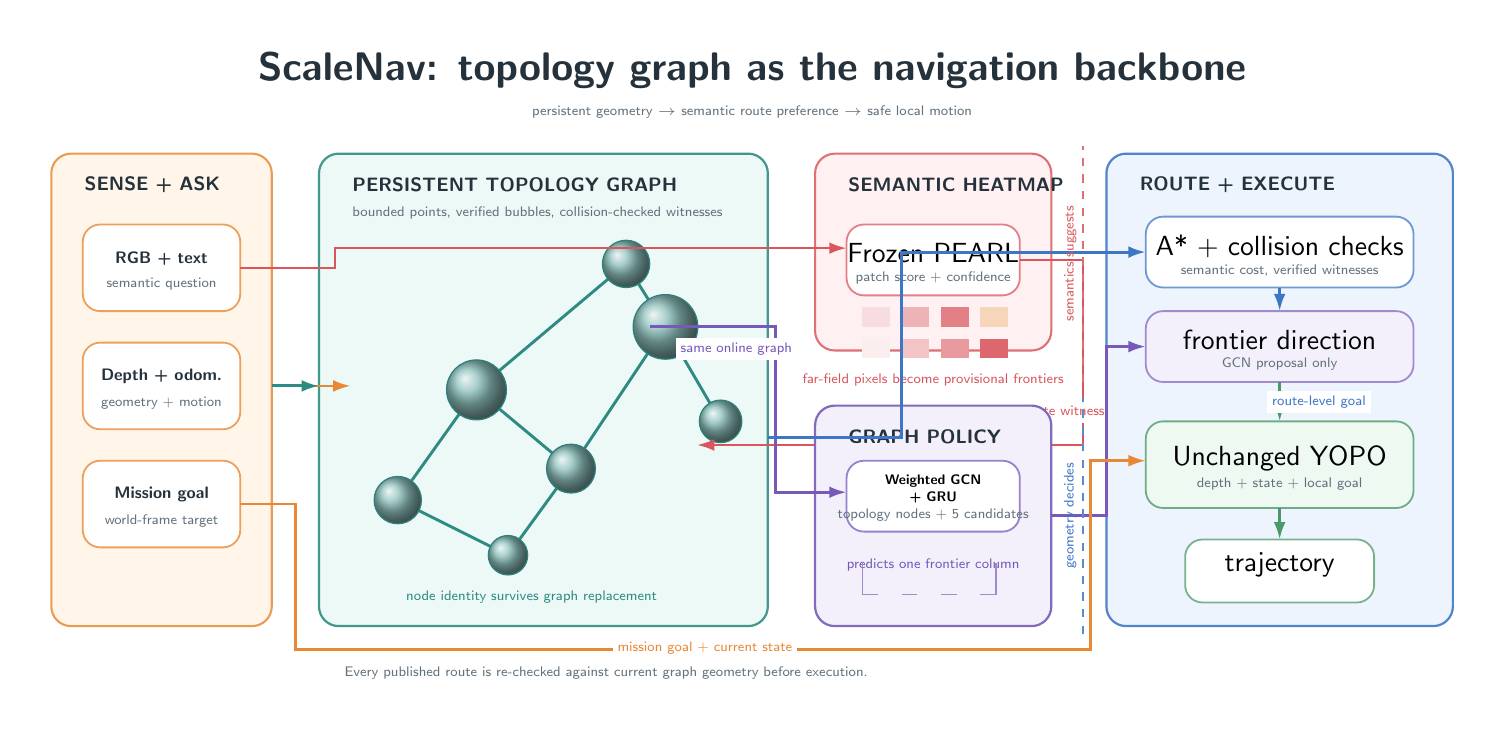
\begin{tikzpicture}[
  x=1mm,y=1mm,font=\sffamily,
  title/.style={font=\sffamily\bfseries\fontsize{15}{17}\selectfont,text=ink},
  group/.style={font=\sffamily\bfseries\fontsize{7.5}{8.6}\selectfont,text=ink},
  box/.style={rounded corners=2.2mm,line width=.65pt,align=center,
              font=\sffamily\bfseries\fontsize{6.7}{7.7}\selectfont,text=ink},
  inputlabel/.style={font=\sffamily\bfseries\fontsize{5.7}{6.5}\selectfont,text=ink,align=center},
  note/.style={font=\sffamily\fontsize{5.1}{6.2}\selectfont,text=muted,align=center},
  flow/.style={-{Latex[length=2.2mm,width=1.5mm]},line width=.9pt,draw=line},
  inFlow/.style={flow,draw=input},
  topoFlow/.style={flow,draw=topo,line width=1.05pt},
  semFlow/.style={flow,draw=sem},
  gcnFlow/.style={flow,draw=gcn,line width=1.05pt},
  planFlow/.style={flow,draw=plan,line width=1.05pt},
  execFlow/.style={flow,draw=exec,line width=1.05pt}
]
\fill[white] (-3,-3) rectangle (181,84);
\node[title] at (89,78.5) {ScaleNav: topology graph as the navigation backbone};
\node[note] at (89,73.3) {persistent geometry  $\rightarrow$  semantic route preference  $\rightarrow$  safe local motion};

% Input lane, with simple icon-like dots for the friendly visual language.
\filldraw[rounded corners=2.5mm,draw=input!85,fill=inputbg,line width=.75pt]
  (0,8) rectangle (28,68);
\node[group,anchor=west] at (3,64) {SENSE + ASK};
\filldraw[box,draw=input!80,fill=white] (4,48) rectangle (24,59);
\node[inputlabel] at (14,54.7) {RGB + text};
\node[note] at (14,51.4) {semantic question};
\filldraw[box,draw=input!80,fill=white] (4,33) rectangle (24,44);
\node[inputlabel] at (14,39.7) {Depth + odom.};
\node[note] at (14,36.3) {geometry + motion};
\filldraw[box,draw=input!80,fill=white] (4,18) rectangle (24,29);
\node[inputlabel] at (14,24.7) {Mission goal};
\node[note] at (14,21.3) {world-frame target};

% Topology graph: bubbles and witness edges are intentionally drawn as a small map.
\filldraw[rounded corners=2.5mm,draw=topo!90,fill=topobg,line width=.8pt]
  (34,8) rectangle (91,68);
\node[group,anchor=west] at (37,64) {PERSISTENT TOPOLOGY GRAPH};
\node[note,anchor=west] at (37,60.5) {bounded points, verified bubbles, collision-checked witnesses};
\draw[topoFlow] (44,24)--(54,38)--(66,28)--(78,46)--(85,34);
\draw[topoFlow] (54,38)--(73,54)--(78,46);
\draw[topoFlow] (44,24)--(58,17)--(66,28);
\foreach \x/\y/\r in {44/24/3.0,54/38/3.8,66/28/3.1,78/46/4.1,85/34/2.7,58/17/2.5,73/54/3.0} {
  \shade[ball color=topo!55!white] (\x,\y) circle (\r mm);
  \draw[topo!90!ink,line width=.45pt] (\x,\y) circle (\r mm);
}
\node[note,text=topo] at (61,11.7) {node identity survives graph replacement};
\draw[inFlow] (28,38.5)--(38,38.5);
\draw[topoFlow] (28,38.5)--(34,38.5);

% Semantic branch enters the graph as provisional, never as certified free space.
\filldraw[rounded corners=2.5mm,draw=sem!85,fill=sembg,line width=.75pt]
  (97,43) rectangle (127,68);
\node[group,font=\sffamily\bfseries\fontsize{6.8}{7.8}\selectfont,anchor=west] at (100,64) {SEMANTIC HEATMAP};
\filldraw[box,draw=sem!75,fill=white] (101,50) rectangle (123,59);
\node at (112,55.4) {Frozen PEARL};
\node[note] at (112,52.2) {patch score + confidence};
\foreach \x/\y/\c in {103/46/sem!20,108/46/sem!45,113/46/sem!75,118/46/input!35,
                         103/42/sem!10,108/42/sem!35,113/42/sem!60,118/42/sem!90} {
  \fill[\c] (\x,\y) rectangle ++(3.5,2.5);
}
\node[note,text=sem] at (112,39.2) {far-field pixels become provisional frontiers};
\draw[semFlow] (24,53.5)--(36,53.5)--(36,56)--(101,56);
\draw[semFlow] (123,54.5)--(131,54.5)--(131,31)--(82,31);
\node[note,text=sem,fill=white,inner sep=.6mm] at (125,35.2) {risk on complete witnesses};

% GCN lane is explicitly graph-native.
\filldraw[rounded corners=2.5mm,draw=gcn!90,fill=gcnbg,line width=.8pt]
  (97,8) rectangle (127,36);
\node[group,anchor=west] at (100,32) {GRAPH POLICY};
\filldraw[box,draw=gcn!75,fill=white] (101,20) rectangle (123,29);
\node[font=\sffamily\bfseries\fontsize{5.5}{6.2}\selectfont,align=center] at (112,25.4) {Weighted GCN\\+ GRU};
\node[note] at (112,22.1) {topology nodes + 5 candidates};
\node[note,text=gcn] at (112,15.8) {predicts one frontier column};
\foreach \x in {103,108,113,118} {\draw[gcn!70,line width=.55pt] (\x,12)--(\x+2,12);}
\draw[gcn!70,line width=.55pt] (103,12)--(103,16);
\draw[gcn!70,line width=.55pt] (120,12)--(120,16);
\draw[gcnFlow] (76,46)--(92,46)--(92,25)--(101,25);
\node[note,text=gcn,fill=white,inner sep=.6mm] at (87,43.2) {same online graph};

% Route and execution lane.
\filldraw[rounded corners=2.5mm,draw=plan!90,fill=planbg,line width=.8pt]
  (134,8) rectangle (178,68);
\node[group,anchor=west] at (137,64) {ROUTE + EXECUTE};
\filldraw[box,draw=plan!75,fill=white] (139,51) rectangle (173,60);
\node at (156,56.3) {A* + collision checks};
\node[note] at (156,53.1) {semantic cost, verified witnesses};
\filldraw[box,draw=gcn!70,fill=gcnbg] (139,39) rectangle (173,48);
\node at (156,44.3) {frontier direction};
\node[note] at (156,41.3) {GCN proposal only};
\filldraw[box,draw=exec!80,fill=execbg] (139,23) rectangle (173,34);
\node at (156,29.3) {Unchanged YOPO};
\node[note] at (156,26.1) {depth + state + local goal};
\filldraw[box,draw=exec!75,fill=white] (144,11) rectangle (168,19);
\node at (156,15.8) {trajectory};
\draw[planFlow] (91,32)--(108,32)--(108,55.5)--(139,55.5);
\draw[gcnFlow] (127,22)--(134,22)--(134,43.5)--(139,43.5);
\draw[planFlow] (156,51)--(156,48);
\draw[execFlow] (156,39)--(156,34);
\draw[execFlow] (156,23)--(156,19);
\draw[inFlow] (24,23.5)--(31,23.5)--(31,5)--(132,5)--(132,29)--(139,29);
\node[note,text=input,fill=white,inner sep=.6mm] at (83,5.2) {mission goal + current state};
\node[note,text=plan,fill=white,inner sep=.6mm] at (161,36.5) {route-level goal};

% Cartoon-style safety boundary and legend.
\draw[sem!85,line width=.9pt,dashed] (131,39)--(131,69);
\node[note,text=sem,rotate=90] at (129.4,54) {semantics suggests};
\draw[plan!85,line width=.9pt,dashed] (131,7)--(131,37);
\node[note,text=plan,rotate=90] at (129.4,22) {geometry decides};
\node[note,anchor=west] at (36,2) {Every published route is re-checked against current graph geometry before execution.};
\end{tikzpicture}
\end{document}
